\documentclass{article}

\usepackage{amsmath}
\usepackage{graphicx}
\usepackage{float}

\title{Moller Event Selection and Kinematics\\at 1.056 GeV}
\date{06-10-2016}
\author{Bradley Yale}

\begin{document}
	\pagenumbering{gobble}
	\maketitle
	\newpage
 	\pagenumbering{arabic}

\section{Introduction}

	\paragraph{}
	Moller scattering is a very useful event to be able to identify in HPS because of its well-known kinematics. This note describes how Moller electrons may be identified using cuts based on the elastic model to isolate them, followed by a production rate comparison between data and Monte Carlo simulations involving Moller events with and without other beam background. Finally, the prospect for correcting the gain calibrations of the ECal edge crystals using selected Moller pairs is introduced and discussed. 
	\paragraph{}
This document is based on 1.05 GeV run conditions, but the same principles apply at any beam energy. This analysis uses Pass3 conditions, which involve the 3.4.1 HPS-Java release and HPS-EngRun2015-Nominal-v3-fieldmap detector geometry. This detector implements a 3D B-field defined in a separate file to match more closely with actual run conditions, as opposed to a constant $By = -0.24 T$.

\section{The Elastic Model}

	\paragraph{}
	Elastic scattering in which an electron scatters from another electron follows a simple model, which relates its energy $E$ to the scattering angle $\theta$:

	\begin{equation}	\label{eq:ET}
  	E(\theta) = \frac{E_{beam}}{1+\frac{2E_{beam}}{m_e}\sin^2{\left(\theta/2\right)}}
	\end{equation}

	In the case of the 2015 Engineering Run, $E_{beam} = \mbox{1.05 GeV}$. The curve which follows this model provides an excellent check of how closely a Moller candidate selected from a collection of vertexed electrons follows the expected scattering model. 
	To minimize accidentals, the primary Moller cuts imposed should involve both electrons selected from a vertexed pair rather than individual electrons, and it will also serve the interest of calibrating with their unique kinematics.

\subsection{Kinematic Interdependence of Moller Electrons}
	\paragraph{}
	Mollers in the HPS experiment should primarily come from a beam electron $\left(E=E_{beam}=\mbox{1.056 GeV}\right)$ that has been scattered from a target electron initially approximated to be at rest. In this case, the energies of the detected Moller pair should always add to the beam energy:

	 \begin{equation} \label{eq:EE}
  	E_2(E_1) = E_{beam} - E_1
	\end{equation}

	Enforcing the condition of elastic scattering, eq.(\ref{eq:ET}), and solving for $\theta_2$, a relationship between the two scattering angles of the Moller pair can be obtained as well:
	
	 \begin{equation} \label{eq:TT}
  	\theta_2(\theta_1) = 2\sin^{-1}{\left(\frac{m_e}{2E_{beam}}\csc{\left(\theta_1/2\right)}\right)}
	\end{equation}

	Together, eqs.(\ref{eq:ET}), (\ref{eq:EE}), and (\ref{eq:TT}) will form the basis for selecting Moller electrons from background physics events. Agreement with this model from pre-SLIC Monte Carlo Mollers is overwhelmingly good, as seen in figures \ref{fig:stdEE}, \ref{fig:stdTT}, and \ref{fig:stdET}.
	
	\begin{figure}[H]
  	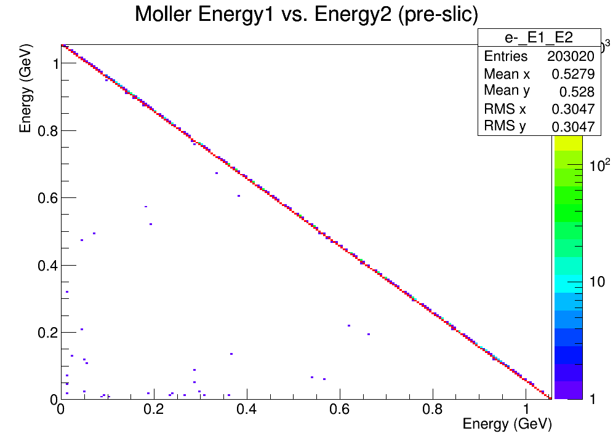
\includegraphics[width=\linewidth]{old/stdEE.png}
  	\caption{$E_1$ vs. $E_2$ of Moller stdhep events just after the target}
  	\label{fig:stdEE}
	\end{figure}
	
	\begin{figure}[H]
  	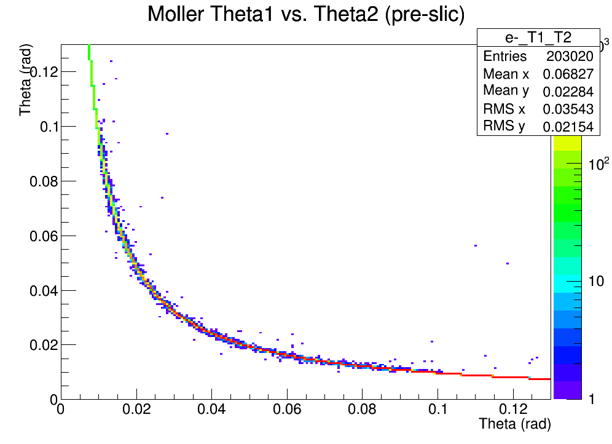
\includegraphics[width=\linewidth]{old/stdTT.png}
  	\caption{$\theta_1$ vs. $\theta_2$ of Moller stdhep events just after the target}
  	\label{fig:stdTT}
	\end{figure}
	
	\begin{figure}[H]
  	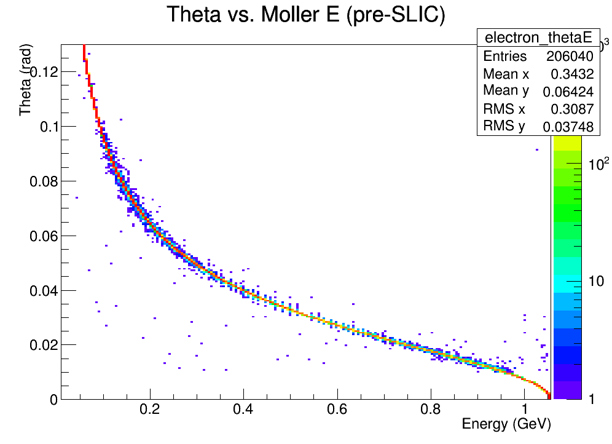
\includegraphics[width=\linewidth]{old/stdET.png}
  	\caption{Energy vs. $\theta$ of Moller stdhep events just after the target. The low-energy tail is due to multiple scattering within the target.}
  	\label{fig:stdET}
	\end{figure}

	From the tails of these distributions, and considering that multiple scattering within the target creates (identifiable) events with photons and positrons, this indicates that only up to 95\% of events using this generator can be confidently identified as Moller events after reconstruction. It is also important to note that all scattering angles used in this study are rotated by $-30.5$ mrad, to undo the beam offset that the simulations also take into account.

	\section{Defining a Class of Moller Selection Cuts}
	\paragraph{}
	'MollerCandidates' is a collection of HpsParticles added for Pass2, which feature vertexed pairs of electrons using the same vertexing procedure as for usual electron-positron pairs, except that the tracks are constrained to both have a negative charge, and hits must be on opposite volumes of the ECal $\left(\tan{\left(\lambda_1\right)}*\tan{\left(\lambda_2\right)}<0\right)$. All analyses will feature these vertexed MollerCandidates with a $\chi^{2}_{vtx}<0.5$ cut for the vertex fit, and $\chi^{2}_{track}<20$ for the track fit. The energies are calculated using the GBL track energy (TrackType$>$32).

	\paragraph{}
	To extract Mollers from data, a bottom-up approach was used to find the selection criteria; Monte Carlo simulations with only scattered Moller events propagated samples of pure Mollers through track reconstruction, electron pairs were vertexed, and primary cuts were made based on (\ref{eq:EE}) and (\ref{eq:TT}), and using the widths of the resulting distributions. These distributions, which quantify the proximity of Mollers to the elastic model, are given in figures \ref{fig:EE}, \ref{fig:TT}, and \ref{fig:ET} for reconstructed pure Monte Carlo MollerCandidates.

	\begin{figure}[H]
  	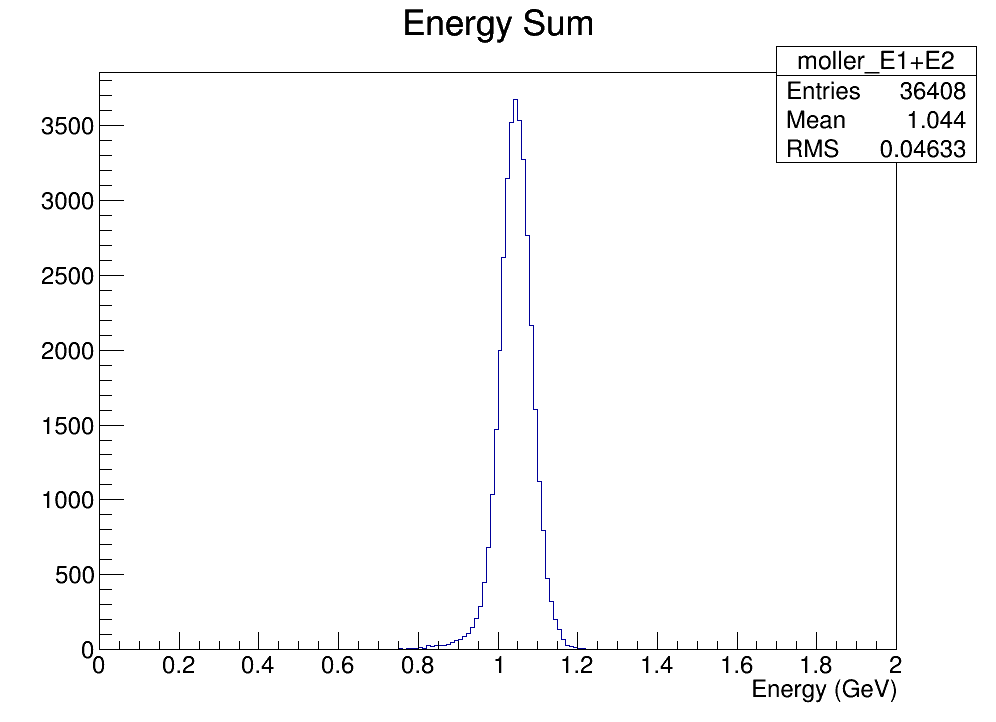
\includegraphics[width=\linewidth]{PostCollabMeet/Pass3PureMoller/RAW_moller_ESum.png}
  	\caption{Distribution showing the proximity of the vertexed Moller pairs to the energy sum condition}
  	\label{fig:EE}
	\end{figure}

	\begin{figure}[H]
  	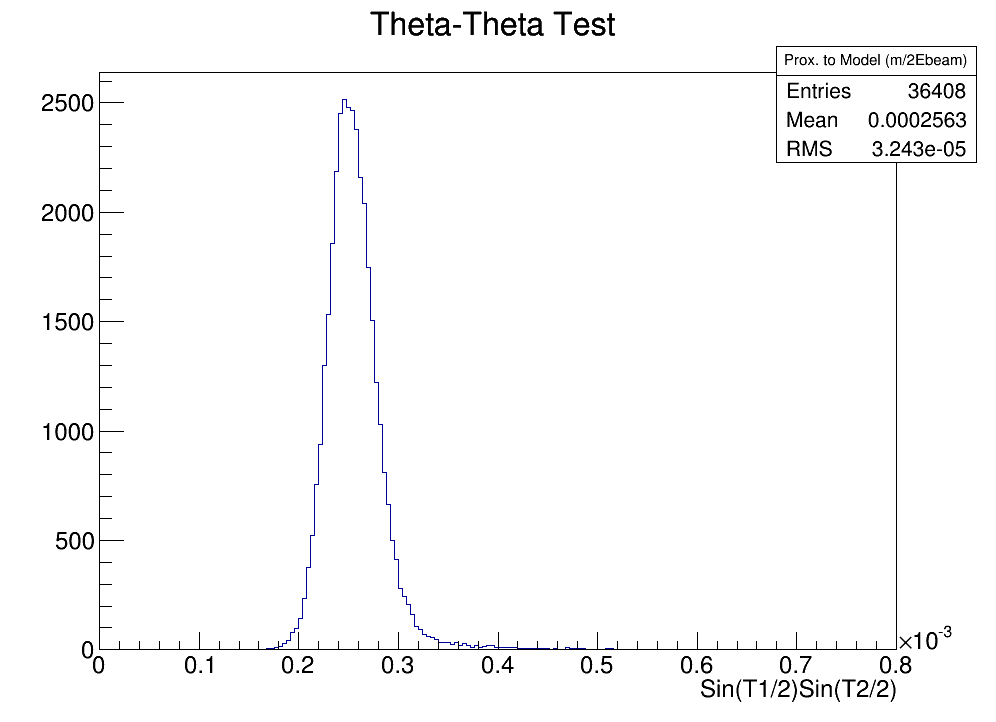
\includegraphics[width=\linewidth]{PostCollabMeet/Pass3PureMoller/RAW_SinSinTest.png}
  	\caption{Distribution showing the proximity of the vertexed Moller pairs to the scattering angle interdependence}
  	\label{fig:TT}
	\end{figure}

	\begin{figure}[H]
  	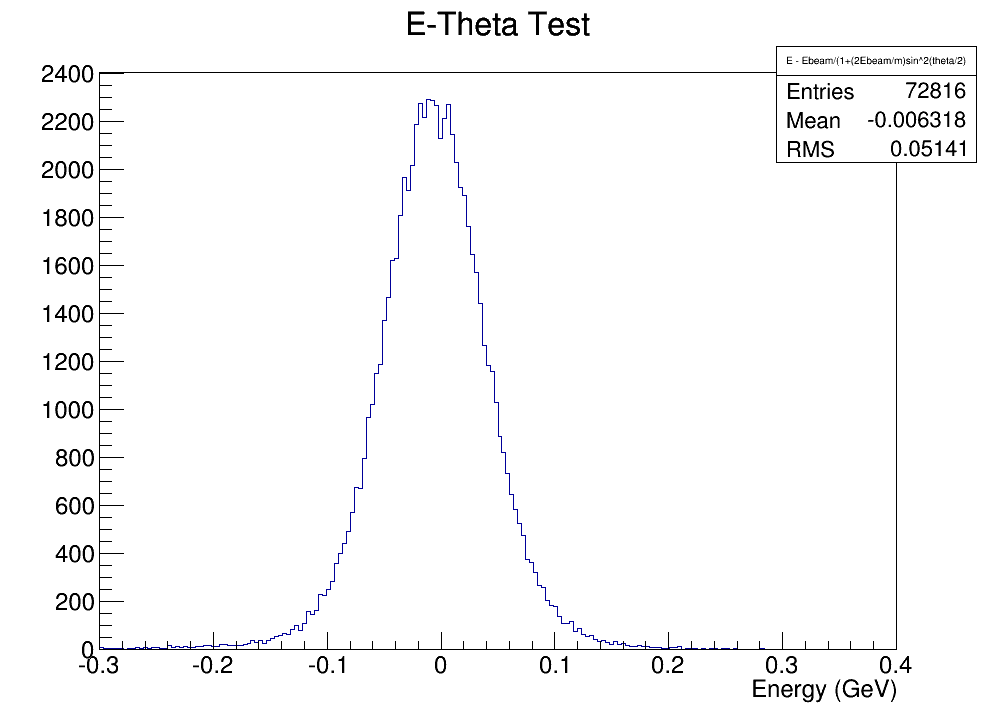
\includegraphics[width=\linewidth]{PostCollabMeet/Pass3PureMoller/RAW_ETTest.png}
  	\caption{Distribution showing the proximity of the track energy of the vertexed Moller pairs to the energy from the elastic model. This defines the best resolution to expect after reconstruction, and so no cuts should be forced beyond it.}
  	\label{fig:ET}
	\end{figure}

	\paragraph{}
	The motivation behind figure \ref{fig:TT} is that $\sin{\left(\theta_1/2\right)}*\sin{\left(\theta_2/2\right)}=\frac{m_e}{2E_{beam}}=2.4*10^{-4}$ provides a constant value to help quantify the proximity of the angular dependence of the Moller pair to the elastic model. Based on these distributions from pure Moller MC, an informed set of primary elastic cuts can be made, using the resolution of the electron-electron curves:
	
	\begin{equation} \label{eq:ESumCut}
  	0.85 GeV\leq E_1+E_2\leq1.25 GeV
	\end{equation}
	
	\begin{equation} \label{eq:SinSinCut}
  	0.00016\leq \sin{\left(\theta_1/2\right)}*\sin{\left(\theta_2/2\right)} \leq0.00045
	\end{equation}
	
	\begin{equation} \label{eq:ETCut}
  	| E_{track}-E_{model}|\leq0.2 GeV
	\end{equation}

	Where $E_{model}$ is the value calculated from eq.(\ref{eq:ET}). These cuts are designed to keep virtually all of the MC Mollers, within the uncertainty of the generated events after the target (95\%). Finding supplemental cuts based on energy and angular distributions of individual Mollers to add to the above, the full set of Moller selection cuts used for this study include:
	
	\begin{equation} \label{eq:TCut}
  	\theta\leq 60 mrad
	\end{equation}
	
	\begin{equation} \label{eq:CoinCut}
  	|Cluster Hit Time_{1} - Cluster Hit Time_{2}| \leq 3 ns
	\end{equation}
	
	\begin{equation} \label{eq:TSumCut}
  	\theta_1+ \theta_2\leq 90 mrad
	\end{equation}\newline
	
	The last cut, eq.(\ref{eq:TSumCut}), is demonstrated in figure \ref{fig:TSumCut}
	
	\begin{figure}[H]
  	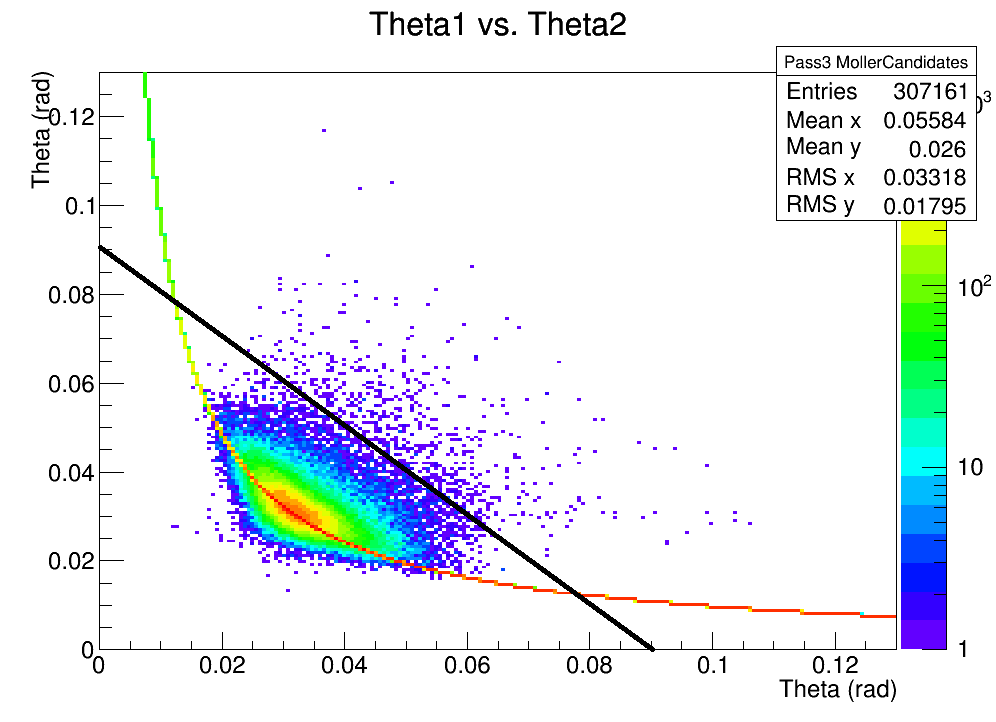
\includegraphics[width=\linewidth]{best_so_far/RAW_mollerTT}
  	\caption{Motivation for the angular sum cut}
  	\label{fig:TSumCut}
	\end{figure}
	
	Applying these cuts to the reconstructed events, the counterparts to figures \ref{fig:stdEE}, \ref{fig:stdTT}, and \ref{fig:stdET} can be found in the Appendices, along with other relevant distributions.
	As a check, the amount of pure Moller events which pass these cuts compared to generated events is
	\begin{equation} \label{eq:efficiency}
	\begin{split}
  	\frac{\mbox{\# of cut Mollers after recon}}{\mbox{\# of uncut Mollers after recon}}
  	= \frac{\mbox{69040}}{\mbox{72816}} = \mbox{94.8\%}
  	\end{split}
	\end{equation}

	This matches the efficiency of the generator, that is, how many Mollers can be confidently identified after the target which may also include some created photons and positrons, but should be present in $<5\%$ of events at this stage. This also indicates that eqs. \ref{eq:ESumCut} - \ref{eq:TSumCut} are effectively the tightest set of cuts of this type that can be performed, while keeping the loss of identifiable Mollers to a minimum. It will be shown that these cuts are too tight to capture all of the accepted Mollers in data, but are useful to ensure that the electrons selected were elastically scattered from one another while eliminating accidental events.

\paragraph{}
It should be noted that, even without any cuts, the Mollers which are ultimately accepted in the ECal and vertexed are taken from the energy range where the Moller production cross section is at a minimum, as seen in figure  \ref{fig:stdE}. The true peaks of the Moller distributions correspond to the electron which is scattered in a forward direction (near the beam energy), and the electron knocked out of the target (low energy). Many of the Moller-scattered beam electrons are actually lost to the electron hole in the ECal, and so the lower-energy Moller electrons which pass geometrical acceptance do not get vertexed. Evidence for this can be seen in studies involving a loose readout trigger and 2.3 GeV Monte Carlo.

	\begin{figure}[H]
  	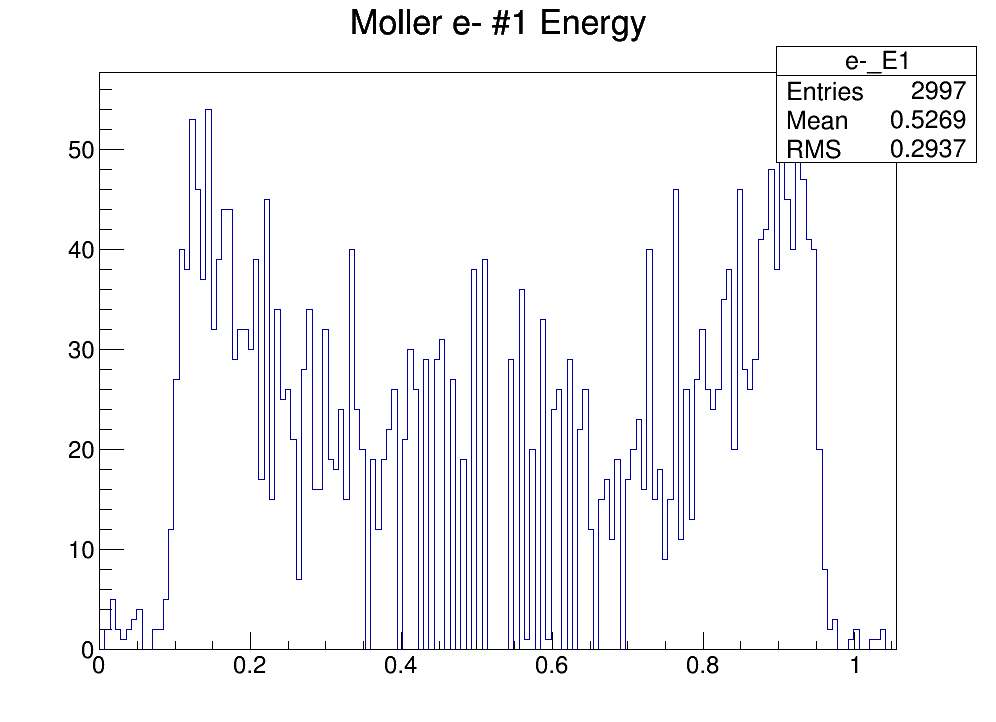
\includegraphics[width=\linewidth]{preSLICmollers/molv1_1700_e-_E1.png}
  	\caption{Energy distribution of Mollers just after the target. The region around Ebeam/2 is the global minimum of the Moller cross section, but is the only region which gets vertexed after reconstruction.}
  	\label{fig:stdE}
	\end{figure}

          \begin{figure}[H]
  	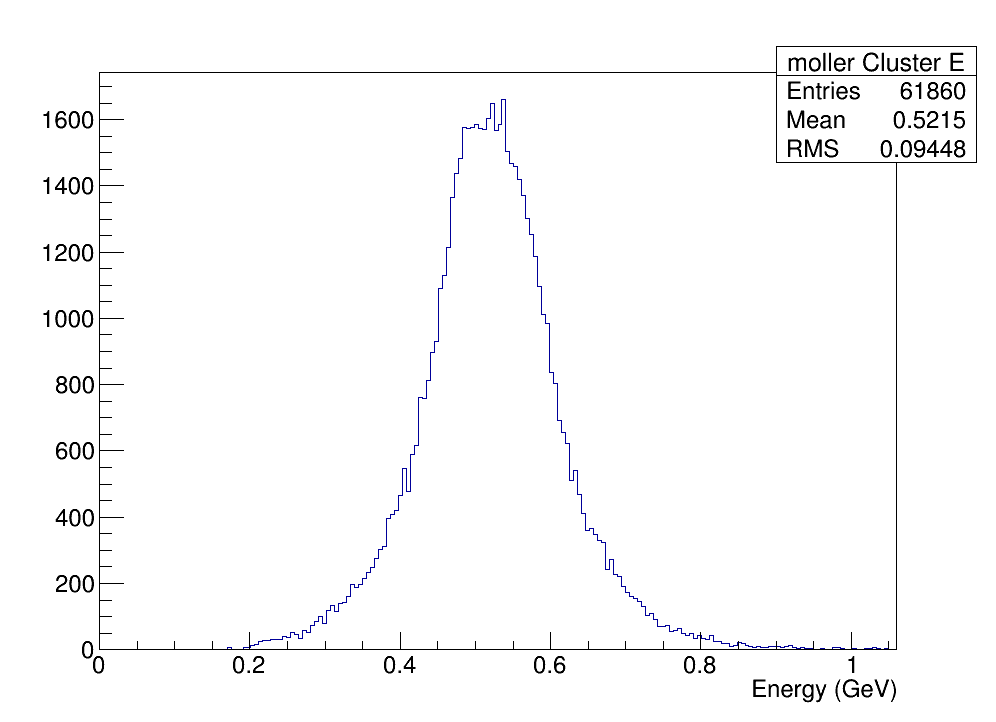
\includegraphics[width=\linewidth]{puremollerMC/RAW_moller_E.png}
  	\caption{GBL track energy of Mollers after reconstruction and vertexing. The region around Ebeam/2 is the global minimum of the Moller cross section, but is the only region which gets vertexed after reconstruction.}
  	\label{fig:reconE}
	\end{figure}

The production rates will be calculated in the next section, based on how much pure Moller MC is accepted, and compared against data. As it turns out, since a large number of Mollers are lost to the electron hole, this significantly reduces the expected number of vertexed 'MollerCandidates' obtained in both MC and data.

	\section{Calculated Moller Production Rates for 1.056 GeV Using Cuts from Monte Carlo}
	\paragraph{}
	In order to test if the cuts propsed in the previous section can be used to correctly extract Mollers from experiment, the rate at which the accepted Mollers are produced should be compared in pure Moller MC, background MC (beam-tri), and data.
	
	\subsection{Moller Production Rate in 1.056 GeV Pure Moller MC}
	\paragraph{}
	It is easy to determine the production rate of Mollers within MC, because 94.8\% of Mollers (or all cut Mollers) can be counted, as well as the number of incident electrons, which have a well-defined time structure of 625 electrons per 2 ns beam bunch (1 event), taken from a current of 50 nA. The number of incident beam bunches used for each pure Moller file is 2M. Therefore, 
	
	\begin{equation} \label{eq:PureRate}
	\begin{split}
  	\mbox{Moller Production Rate in Pure Moller MC} = \frac{(\mbox{generator efficiency})(\mbox{\# of events before readout})}{\mbox{time}} \\
  	= \frac{(0.948)(34761)}{(\mbox{10 files})(\mbox{2M bunches/file})(\mbox{2ns/bunch})}\\= \mbox{823835.7 Hz}
  	\end{split}
	\end{equation}
	
	In addition, the acceptance for reconstructed Mollers with these cuts can be obtained, for the purpose of normalizing the rates from data:
	\begin{equation} \label{eq:MollerAcceptance}
	\begin{split}
  	\mbox{Cut Moller Acceptance} = \frac{\mbox{\# of cut Mollers after recon}}{\mbox{\# of uncut Mollers before readout}} \\
  	= \frac{34520\mbox{ Moller events}}{(\mbox{300 recon files})(\mbox{34761 pre-readout events})}\\ = \mbox{0.331\%}
  	\end{split}
	\end{equation}

	This is an extremely low acceptance for reasons mentioned in the previous section. This acceptance also factors in those events lost from only selecting a restrictive subset of cut GBL tracks, and should therefore only be used for analyses involving the same $\chi^{2}$ cuts.

	\subsection{Moller Production Rate in Beam-Tri MC}
	\paragraph{}
	The usual Monte Carlo that represents the full background in which the A' will be searched is 'beam-tri', which contains QED tridents (radiative and Bethe-Heitler), hadrons, and scattered beam, the last of which contains the Moller scattering process. To see if this vital MC component has the correct Moller production rate, the same well-known time structure can be used:
	
	\begin{equation} \label{eq:BeamTriRate}
	\begin{split}
  	\mbox{Moller Production Rate in Background MC} =\frac{(\mbox{generator efficiency})(\mbox{\# of cut Moller events after recon})}{\mbox{(time)({acceptance factor})}} \\
  	= \frac{(0.948)(3113\mbox{ cut Moller events})(0.00331)^{-1}}{(\mbox{111 recon files})(\mbox{10 SLIC files})(\mbox{500k events/file})(\mbox{2ns/event})}\\= \mbox{803223.65 Hz}
  	\end{split}
	\end{equation}
	
	From this, the rate of Moller production in pure Moller MC differs from the full beam background simulation by \mbox{2.5\%}

	\subsection{Moller Production Rate in Data}
	\paragraph{}
	Using the cuts from pure Moller MC, as well as the calculated acceptance factor from eq.(\ref{eq:MollerAcceptance}), and taking into account the known Moller acceptance from the singles1 trigger of \mbox{2.269\%}, the Moller production rate from data can be obtained. The time that was used in eq.(\ref{eq:DataRate}) was calculated using the total charge taken from the MYA Faraday cup values of all unblinded run 5772 files (Pass3), corrected for livetime, SVT bias, and SVT position, and using a current of \mbox{50 nA}.
	
	\begin{equation} \label{eq:DataRate}
	\begin{split}
  	\mbox{Moller Production Rate in Data}= \frac{\mbox{\# of cut Moller events after recon}}{(\mbox{time})(\mbox{acceptance factors})}\\
  	= \frac{(\mbox{17344})(0.00331)^{-1}}{(\mbox{570.56s})\mbox{(0.948)(0.02269)}}\\= \mbox{428460 Hz}
  	\end{split}
	\end{equation}
	
According to this, the number of Moller events in data appears to be half of what is found in Monte Carlo, with or without background present; this still appears to be the case when normalizing the respective plots by luminosity, using eq.(\ref{eq:Lumin}) from the next section. In an effort to help explain this, the full run 5772 pass3 data represented above was normalized by luminosity and compared before and after the cuts. From this, it seems that the previous cuts based on the MC are too tight, and do in fact remove half of the Moller peak in data, if the height of the peaks are examined (figures \ref{fig:UncutNormData} and \ref{fig:CutNormData}).

\begin{figure}[H]
  	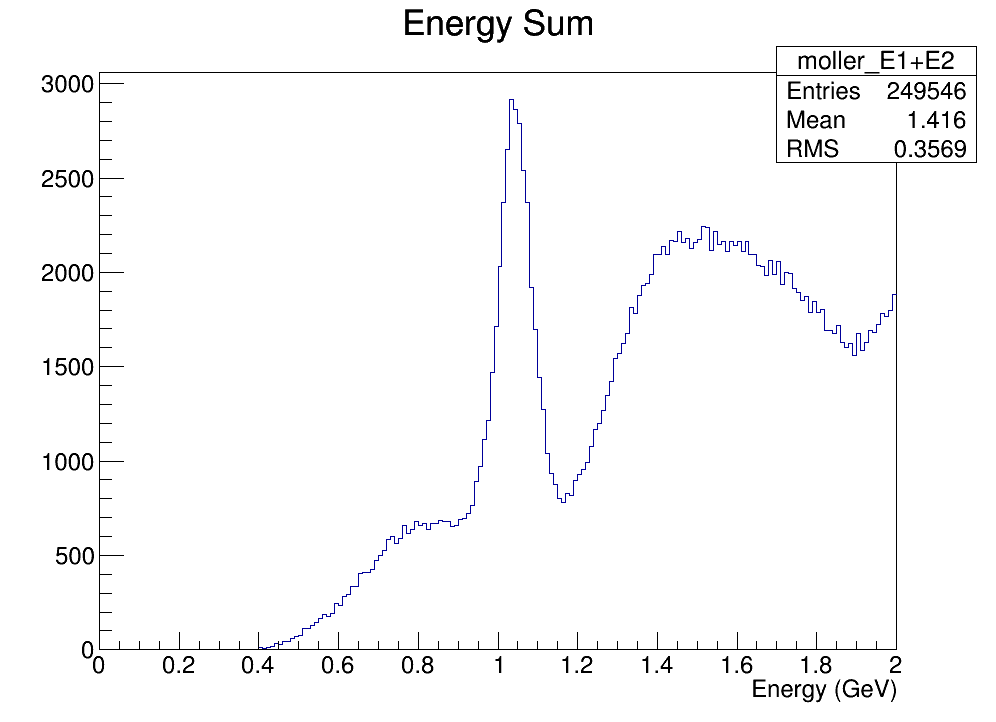
\includegraphics[width=\linewidth]{PostCollabMeet/Pass3Data/Full5772/RAW_moller_ESum.png}
  	\caption{Energy sum peak of vertexed electrons in data with no further cuts}
  	\label{fig:UncutNormData}
	\end{figure}

\begin{figure}[H]
  	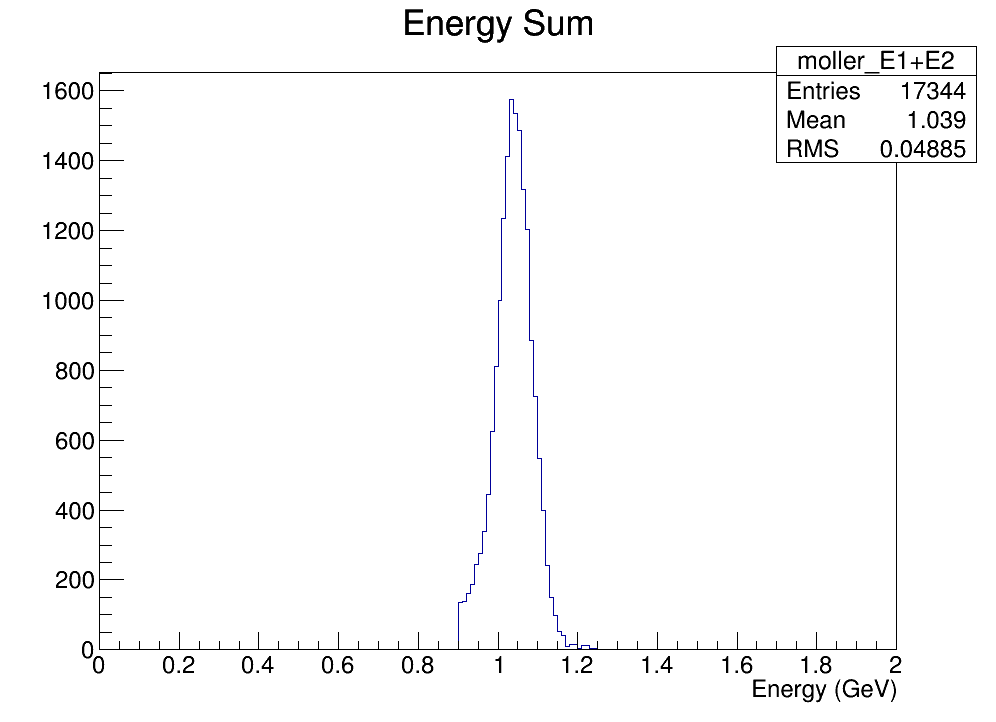
\includegraphics[width=\linewidth]{PostCollabMeet/Pass3Data/Full5772/CUT_TestEE.png}
  	\caption{Energy sum peak of vertexed electrons in data with the same cuts used to get the events for the rate calculations. The peak maintains its narrow width, but the height is reduced by roughly half, which agrees with the rate calculation.}
  	\label{fig:CutNormData}
	\end{figure}

This suggests that the resolutions of the various Moller plots created with GBL tracks may be worse for data, and the actual cuts to be used must be quite looser than those proposed above. In the following section, agreement between MC and data will be further explored by fitting the uncut vertexed electrons in data, and comparing the extracted Gaussian part of that fit with the normalized Monte Carlo signal.

\subsection{Fitting the Moller background}
	\paragraph{}
	In an effort to further understand and compare the Moller rates between MC and data, the energy sum peak for the vertexed electrons in otherwise uncut data was fit to a Gaussian + 3rd degree polynomial, shown in figure \ref{fig:BGFit}.

	\begin{figure}[H] 
  	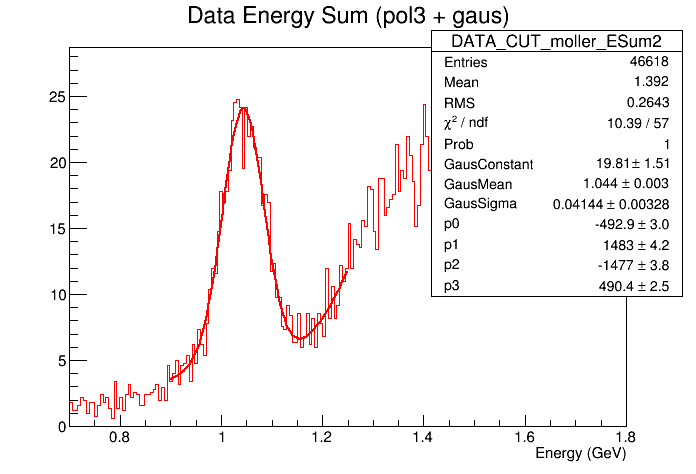
\includegraphics[width=\linewidth]{DataPolGaus.png}
  	\caption{Gaussian + Polynomial fit of the vertexed electron peak in data}
	\label{fig:BGFit}
	\end{figure}

	Once this fit was performed, the Gaussian part was taken to be the Moller signal and compared against a Gaussian fit to the energy sum peak of pure Mollers in Monte Carlo. The resulting Gaussians are compared in figure \ref{fig:DataMCFit}.
 
	\begin{figure}[H]
  	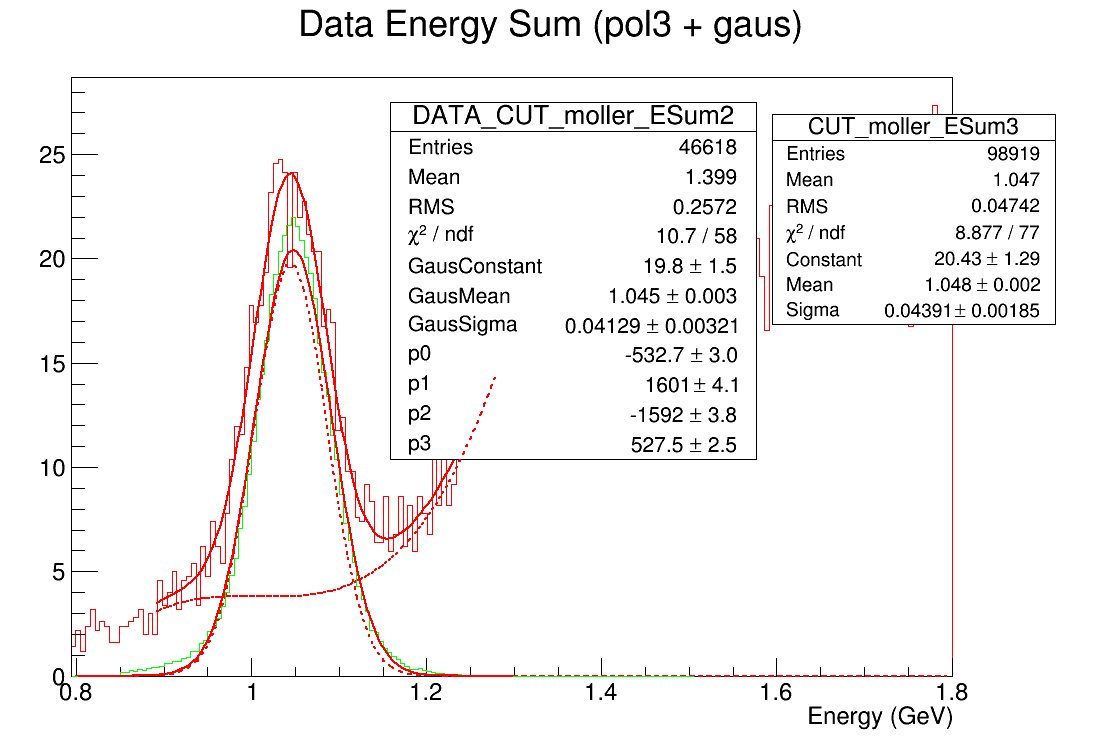
\includegraphics[width=\linewidth]{c1.png}
  	\caption{Comparison of signal fits between data and MC. The red distribution is uncut MollerCandidates from the full run 5772 of pass3 data, the green distribution is pure Moller MC, and the dashed lines are the Gaussian and polynomial parts of the background fit of figure \ref{fig:BGFit}. The solid red lines are the total respective fits of the distributions.}
  	\label{fig:DataMCFit}
	\end{figure}

These distributions were normalized by luminosity so that the areas under the peaks correspond to the respective cross sections. The equation used for the luminosities is given by:

	\begin{equation} \label{eq:Lumin}
	\begin{split}
  	\mbox{Luminosity} = \frac{N_e*\rho*\mbox{(target thickness)}*N_A}{\mbox{atomic weight of tungsten}}\\
  	= \frac{N_e*(\mbox{19.6 }g/cm^{3})*(6.022*10^{23})}{\mbox{183.84 g/mol}}
  	\end{split}
	\end{equation}

Here, $N_e$ is the number of incident electrons hitting the target. For MC, this number is simply calculated by $\mbox{(\# of files )}*\mbox{(\# of electrons per beam bunch)}*\mbox{(\# of beam bunches)}$. For data, the number of incident electrons is obtained from the gated Faraday cup charge, corrected for livetime, SVT bias, and SVT position. In addition, the normalization takes into account the singles1 trigger prescale of $2^{11} = 2048$, which is absent for Monte Carlo (the prescale is set to '1'). While the exact events that fall under the Gaussian in the data cannot be directly tested against the Moller models, this demonstrates that, assuming a signal + Gaussian model for the background yields a normalized signal that is very close in shape and position to what is expected based off pure Moller Monte Carlo; specifically, the positions of the peaks vary by 0.28\%, and the heights by 3\%. The discrepancy in the rates from the previous section must then be due to assuming the same resolutions between Monte Carlo and experiment.

	\section{Mollers for Edge Crystal Calibration}
	\paragraph{}
	The inner edge crystals adjacent to the opening of the ECal are known to be less reliable when calibrated with full-energy electrons relative to the so-called 'fiducial region' which excludes them, due to a higher energy loss of the particles which hit the edge, as seen in figures \ref{fig:EPEdge} and \ref{fig:EPFiducial}. 
	
	\begin{figure}[H]
  	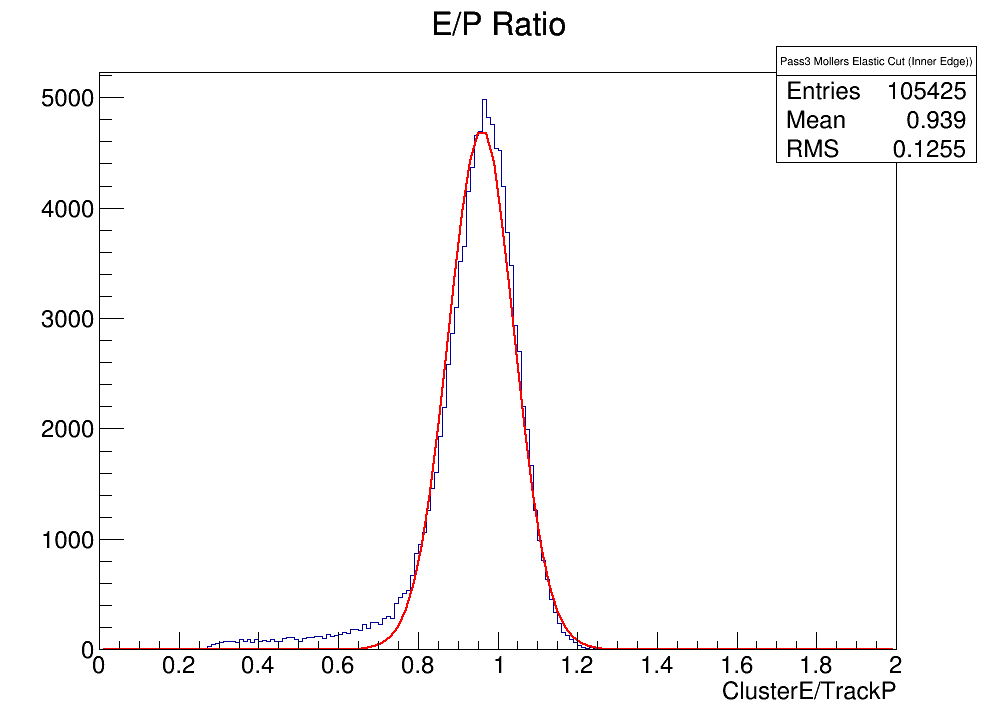
\includegraphics[width=\linewidth]{PostCollabMeet/Pass3PureMoller/EDGE_MollerEPRatio.png}
  	\caption{Ratio of GBL track momentum and ECal cluster energy of pure Moller MC, with seed hits constrained to be on the edge crystals}
  	\label{fig:EPEdge}
	\end{figure}
	
	\begin{figure}[H]
  	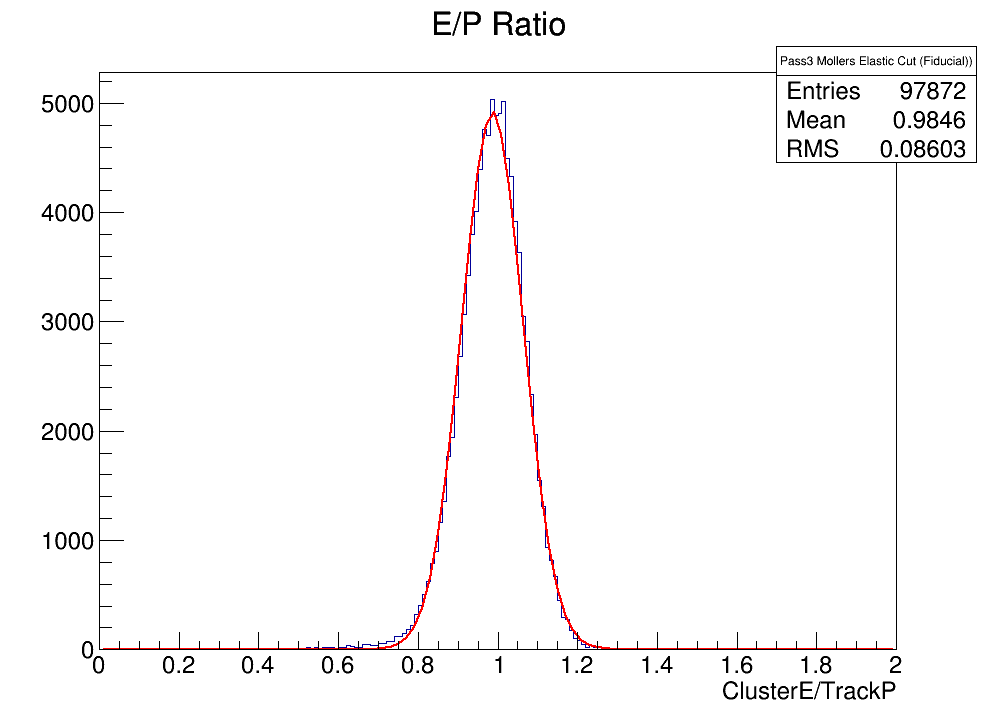
\includegraphics[width=\linewidth]{PostCollabMeet/Pass3PureMoller/FIDUCIAL_MollerEPRatio.png}
  	\caption{Ratio of GBL track momentum and ECal cluster energy of pure Moller MC, with seed hits constrained to be within the fiducial region (all crystals except for those along the inner edge)}
  	\label{fig:EPFiducial}
	\end{figure}
	
	If Moller electrons can be confidently identified, then one potential application would be to find vertexed and cut Moller pairs which have one seed hit in the well-calibrated fiducial region, and one Moller in an edge crystal, and then correcting the gains in the edge crystal with the 	calculated energy using the fiducial Moller. Figures \ref{fig:hits} and \ref{fig:calibHits} show respectively the ECal coverage of the cut Mollers from the above pure Moller MC analysis (eqs. \ref{eq:ESumCut} - \ref{eq:TSumCut}), and those pairs which pass the condition of having fiducial+edge hits.

	\begin{figure}[H]
  	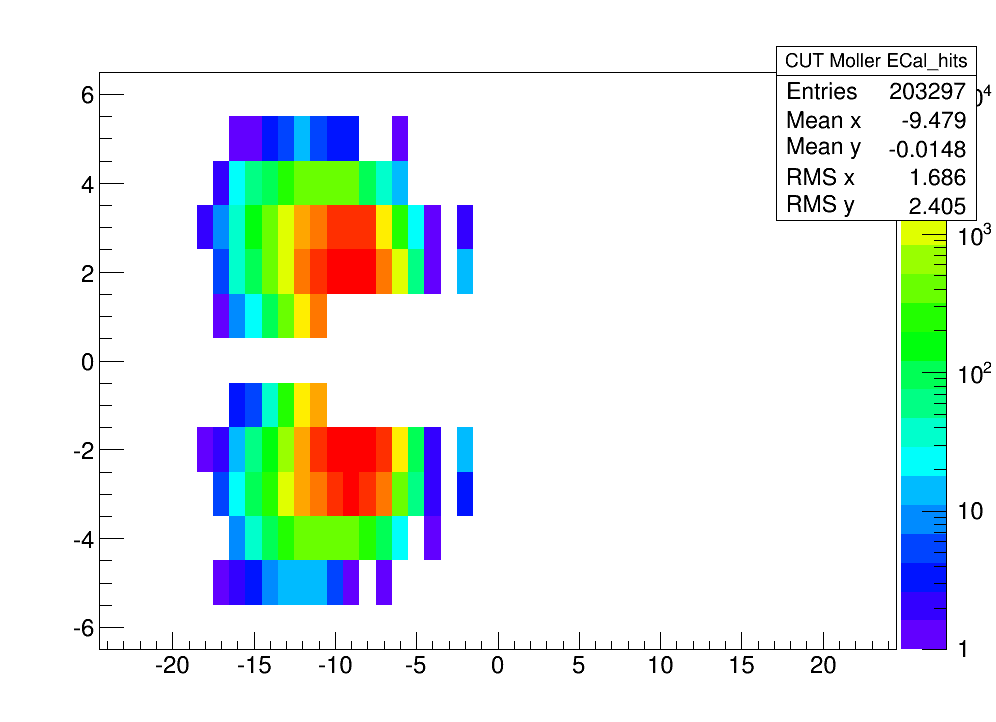
\includegraphics[width=\linewidth]{PostCollabMeet/Pass3PureMoller/CUT_ECal_hits.png}
  	\caption{ECal coverage of Moller electrons with the proposed cuts}
  	\label{fig:hits}
	\end{figure}
	
	\begin{figure}[H]
  	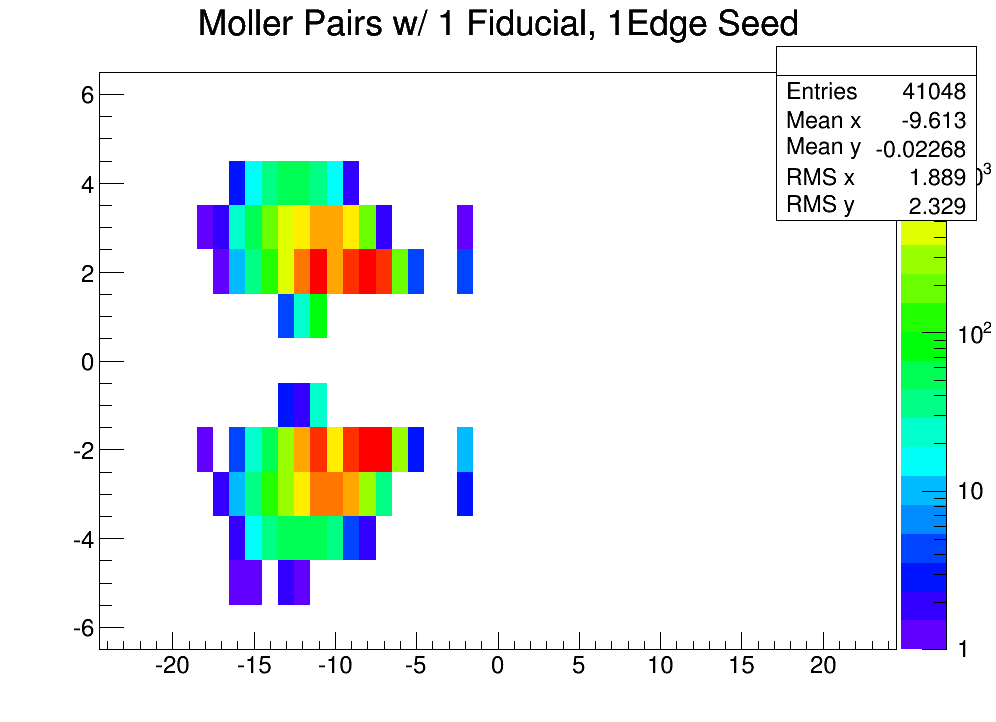
\includegraphics[width=\linewidth]{PostCollabMeet/Pass3PureMoller/CUT_ECalMollers4Calib.png}
  	\caption{ECal coverage of Moller electrons with the proposed cuts, having one fiducial hit and one edge hit}
  	\label{fig:calibHits}
	\end{figure}
	
	This demonstrates that, with tight $\chi^{2}$ cuts on both vertex and track fits, $\sim$20\% of Mollers collected at the $\sim$810 kHz rate found in MC and data can be used for edge corrections. For a typical 1.6 hour run, and considering the calculated acceptance, this translates to $\sim$300k Mollers per run that can be used for edge calibrations. Depending on the need for statistics, the tight $\chi^{2}_{vtx}<0.5$ cut may possibly be loosened in the future without an appreciable loss of quality. What should also be considered when analyzing calibration prospects is that the already low Moller statistics in a narrow energy range hit an equally narrow region of the ECal. This exact region changes slightly based on the beam energy, and so both 1.056 GeV and 2.2 GeV Mollers can be used for calibrating slightly different regions.
	
	\section{Summary}
	\paragraph{}
	This note demonstrates that, while elastic cuts based off Monte Carlo are useful in principle to extract Mollers in data, the actual cuts need to be looser than what is suggested based off Monte Carlo distributions. This conclusion is drawn from a decrease in calculated and observed Moller yields between data and Moller Monte Carlo by roughly half when assuming the same resolutions in data and Monte Carlo. However, when extracting the Moller signal from the normalized background without any cuts and comparing against Monte Carlo, the signals agree very well, with a 3\% difference in peak height, 6\% difference in $\sigma$, and $<$ 1\% difference in peak position. This suggests that the Moller yield in data may be correct, but one must understand the resolution differences between MC and experiment very well when selecting cuts to extract them. Any Mollers that are extracted from data can then be tested using the elastic models, once the beam offset is accounted for.
	\paragraph{}
Even so, while Monte Carlo and data appear to be in agreement, the Mollers that are actually collected and vertexed within HPS are taken from the energy range where the Moller cross section is at its minimum, at $E_{beam}/2$. This is the likely reason why the Moller acceptance is found to be extremely low relative to what is produced in the target $\left(\sim0.3\%\right)$, and likewise occupy a relatively small region of the ECal due to a narrow energy range, translating to an equally narrow acceptance since the range of scattering angles is also restricted.
	\paragraph{}
	With the caveat mentioned above, the energy-momentum correlation of extracted Moller pairs can potentially be used for a variety of calibration purposes. One potential application would be to use Moller pairs with hits divided between the fiducial and edge regions of the ECal to calculate the gains of the edge crystals, thereby making the resolutions across the face of the ECal more uniform. The feasibility of this type of calibration was shown, with an estimated 300k Moller events accepted for a typical run, which matches the number of raw events taken from a file of 'beam-tri' MC, which is the source of the full-energy electrons normally used for calibrations in that energy regime. Since Moller energy peaks at half the beam energy, this would also be a valuable check against the high-energy FEE regime, and calibrations which use low-energy cosmic events.
	
	\section{Appendix A: Pure Moller distributions at 1.056 GeV}
	
	\begin{figure}[H]
  	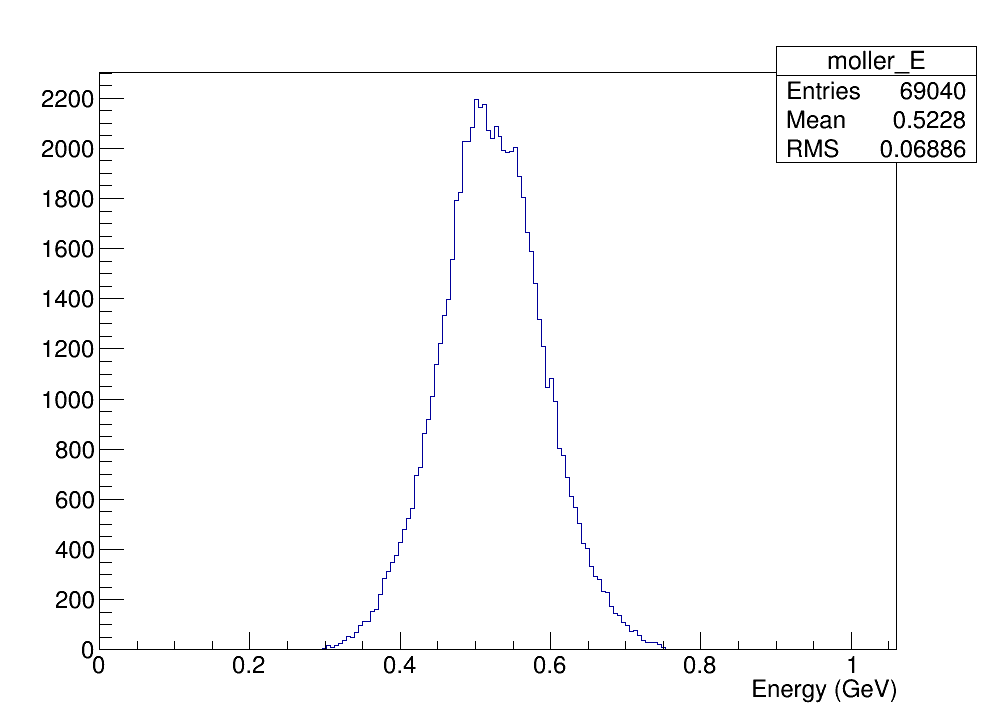
\includegraphics[width=\linewidth]{PostCollabMeet/Pass3PureMoller/CUT_moller_E.png}
  	\caption{Energy of cut Moller events after reconstruction}
  	\label{fig:cutE}
	\end{figure}
	
	\begin{figure}[H]
  	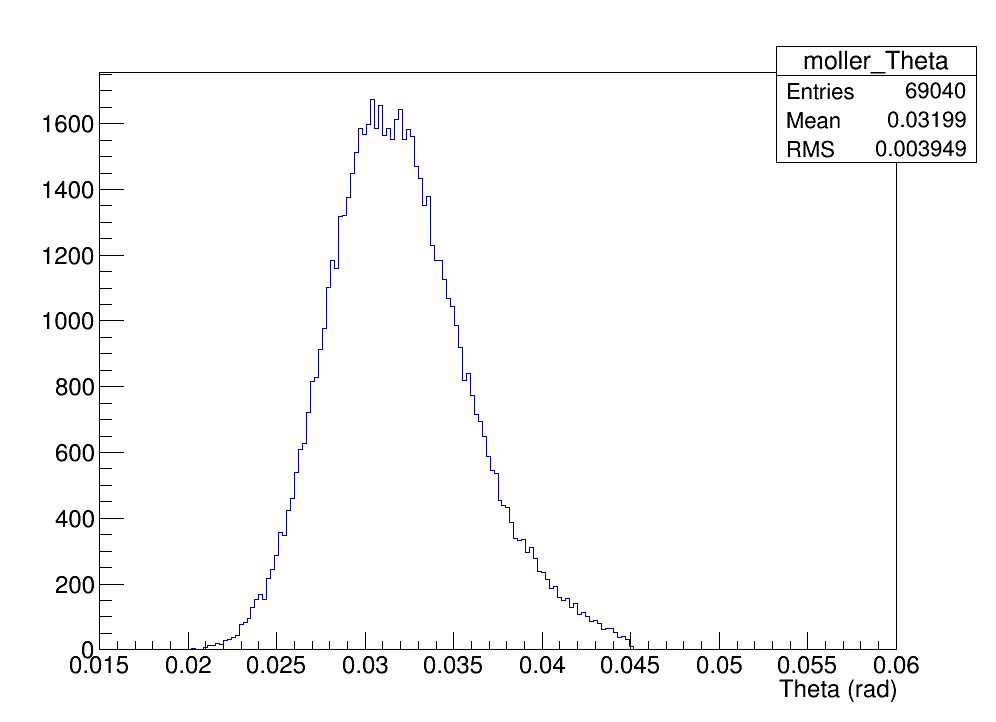
\includegraphics[width=\linewidth]{PostCollabMeet/Pass3PureMoller/CUT_moller_Theta.png}
  	\caption{Scattering angle (theta with -30.5 mrad rotation) of cut Moller events after reconstruction}
  	\label{fig:cutT}
	\end{figure}
	
	\begin{figure}[H]
  	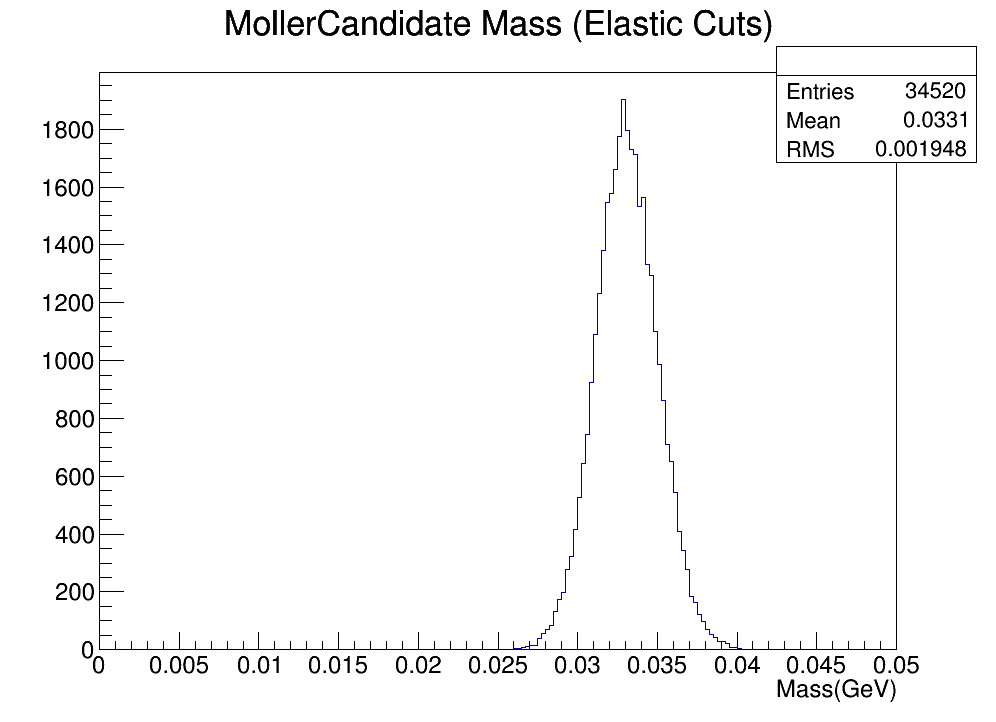
\includegraphics[width=\linewidth]{PostCollabMeet/Pass3PureMoller/CUT_InvarMass.png}
  	\caption{Invariant mass of cut Moller events after reconstruction}
  	\label{fig:cutMass}
	\end{figure}
	
	
	\begin{figure}[H]
  	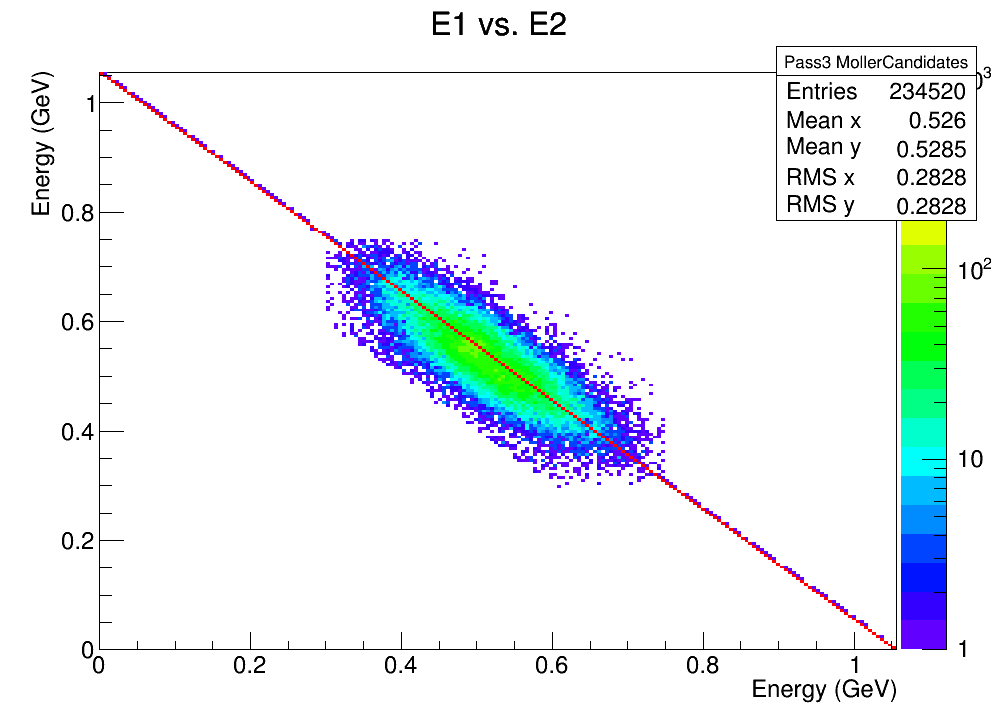
\includegraphics[width=\linewidth]{PostCollabMeet/Pass3PureMoller/CUT_PlotEE.png}
  	\caption{$E_1$ vs. $E_2$ of cut Moller events after reconstruction}
  	\label{fig:cutEE}
	\end{figure}
	
	\begin{figure}[H]
  	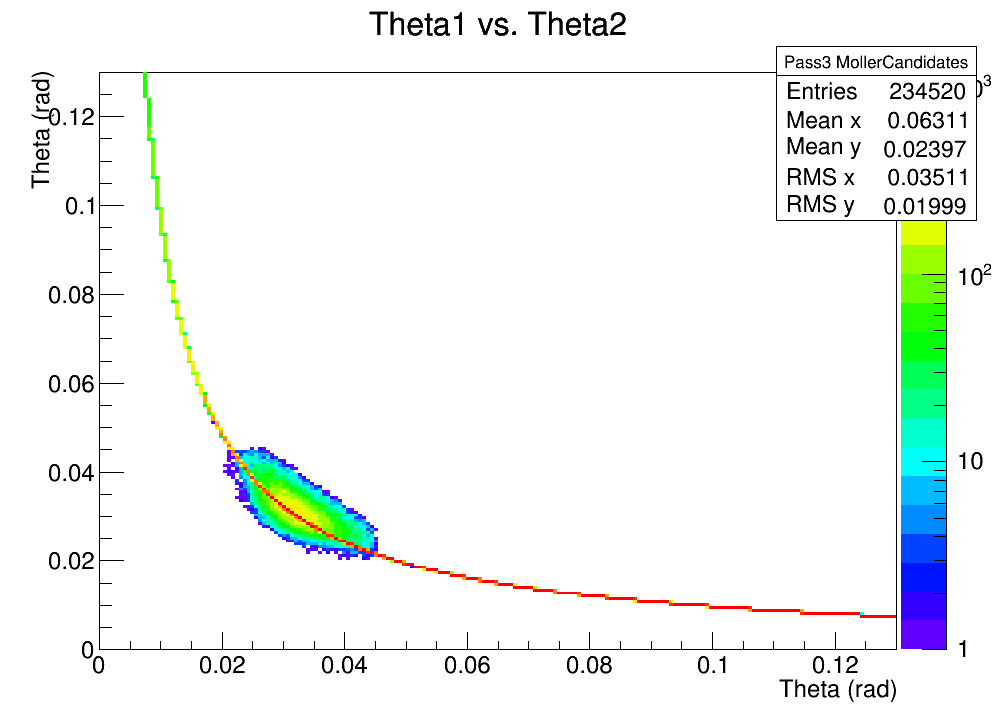
\includegraphics[width=\linewidth]{PostCollabMeet/Pass3PureMoller/CUT_PlotTT.png}
  	\caption{$\theta_1$ vs. $\theta_2$ of cut Moller events after reconstruction}
  	\label{fig:cutTT}
	\end{figure}
	
	\begin{figure}[H]
  	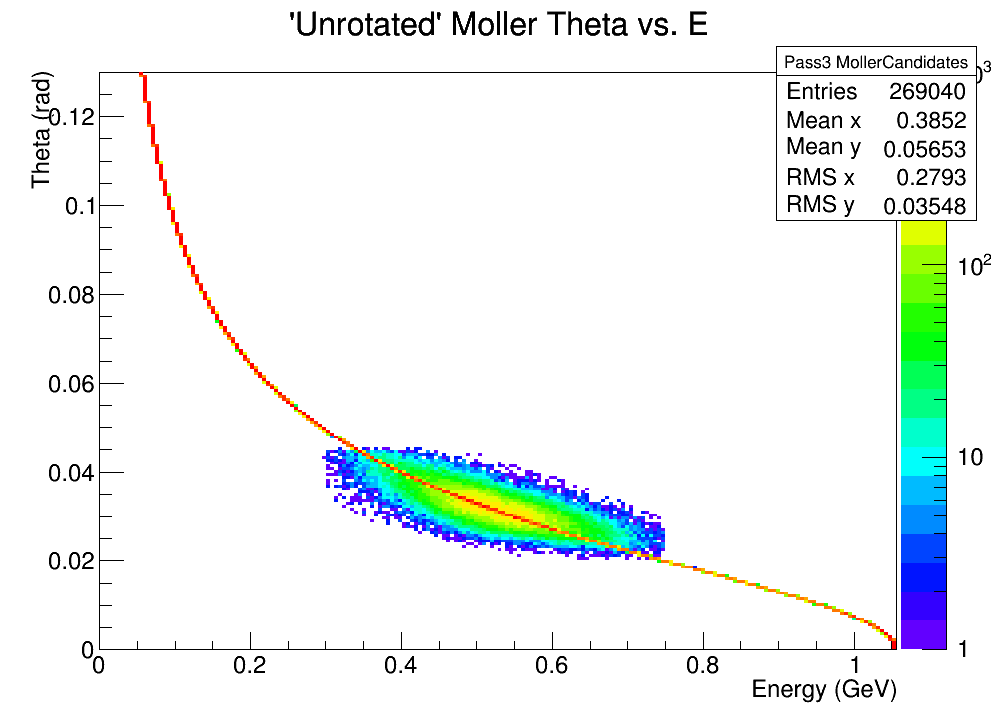
\includegraphics[width=\linewidth]{PostCollabMeet/Pass3PureMoller/CUT_Unrotmoller_ThetaE.png}
  	\caption{Energy vs. $\theta$ of cut Moller events after reconstruction.}
  	\label{fig:cutET}
	\end{figure}
	
	\section{Appendix B: Cut Moller Distributions from Data}
	
	\begin{figure}[H]
  	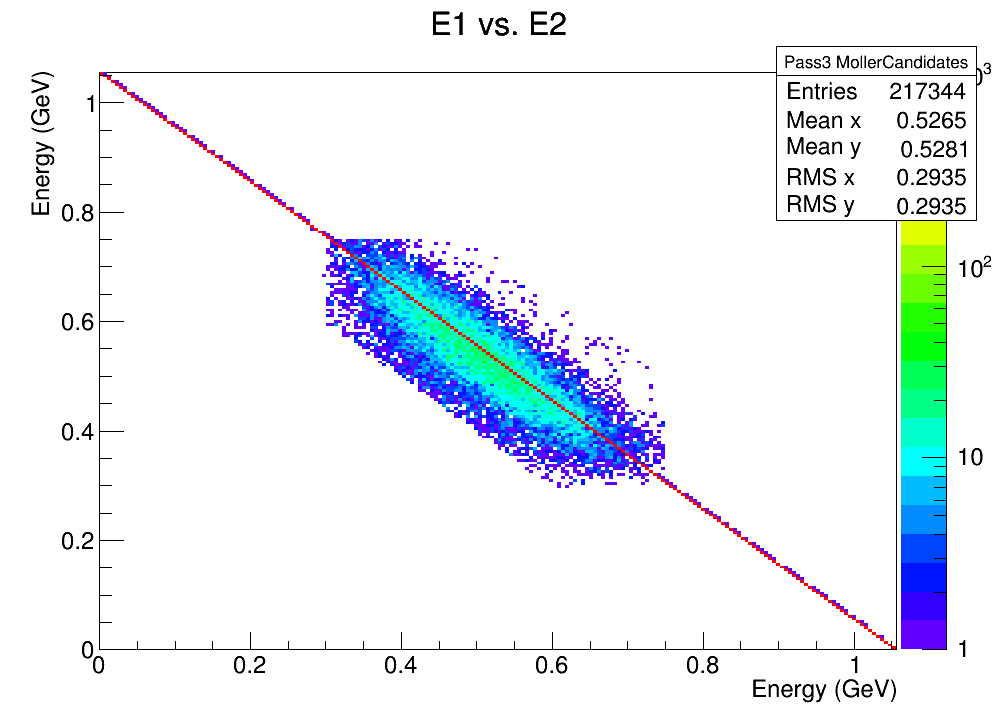
\includegraphics[width=\linewidth]{PostCollabMeet/Pass3Data/Full5772/CUT_PlotEE.png}
  	\caption{$E_1$ vs. $E_2$ of cut Moller events after reconstruction}
  	\label{fig:cutDataEE}
	\end{figure}
	
	\begin{figure}[H]
  	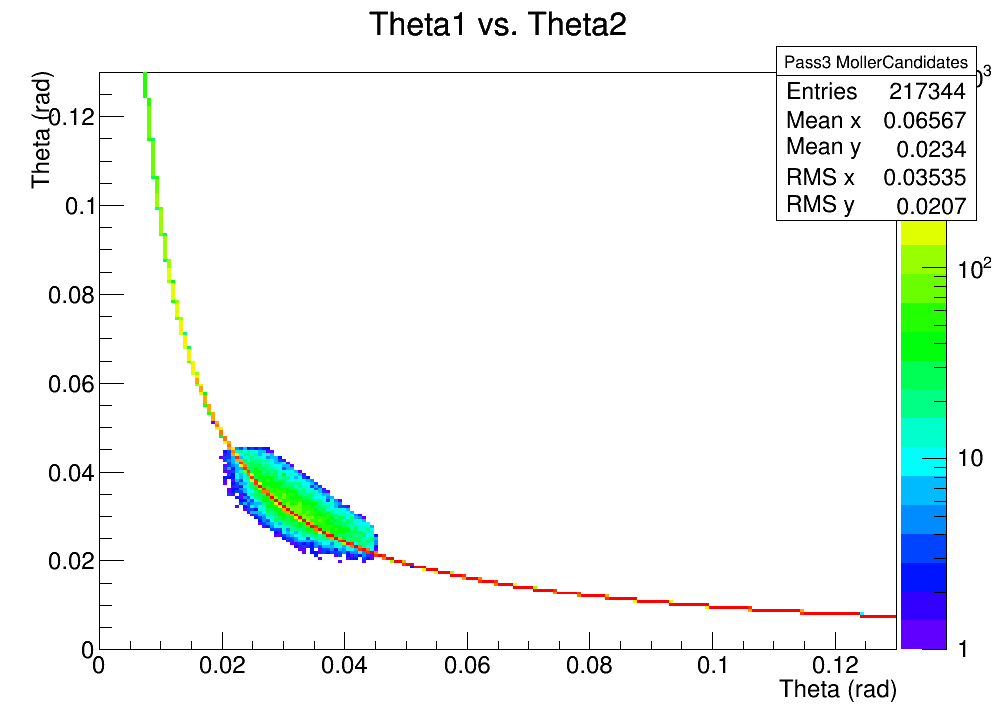
\includegraphics[width=\linewidth]{PostCollabMeet/Pass3Data/Full5772/CUT_PlotTT.png}
  	\caption{$\theta_1$ vs. $\theta_2$ of cut Moller events after reconstruction}
  	\label{fig:cutDataTT}
	\end{figure}
	
	\begin{figure}[H]
  	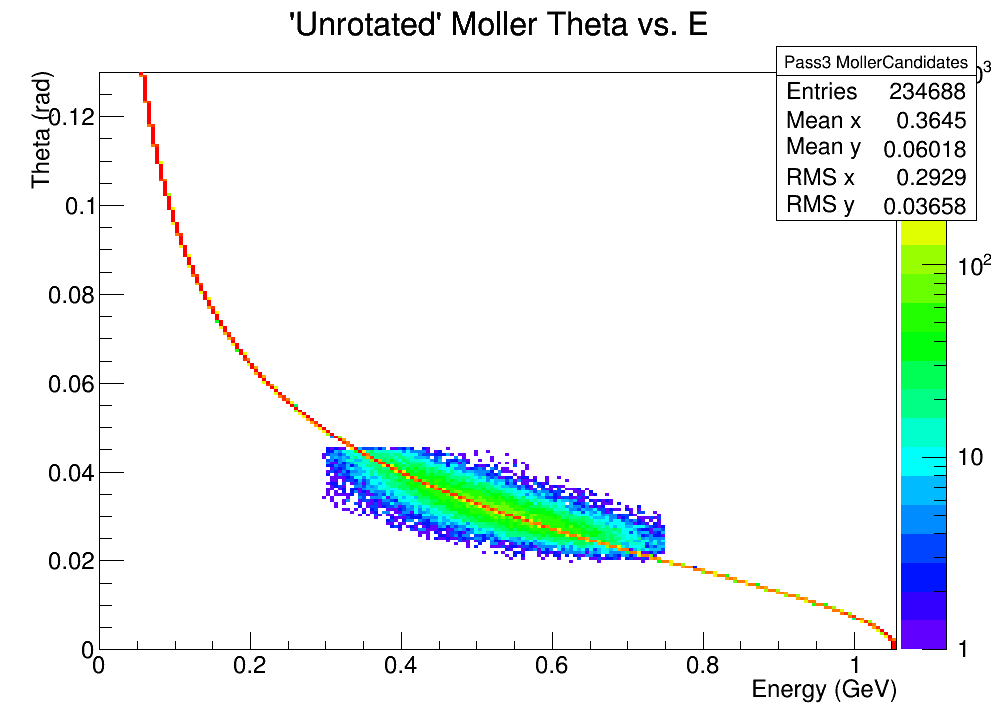
\includegraphics[width=\linewidth]{PostCollabMeet/Pass3Data/Full5772/CUT_Unrotmoller_ThetaE.png}
  	\caption{Energy vs. $\theta$ of cut Moller events after reconstruction.}
  	\label{fig:cutDataET}
	\end{figure}

\end{document}